% Chapter Template
\chapter{Theoretical study of Turing patterns }
\section{Synopsis}
When studying regular pattern formation in biology, Turing patterns are a commonly used mechanism.
Studying Turing patterns can be done both using linear stability analysis or numerical methods.
Linear stability analysis predicts whether a pattern will occur through a dispersion relation.
Although faster, this method provides less insights into the pattern that emerges, as it relies on the linearisation around the steady state.
On the other hand numerical methods, which are more computationally expensive, provide a result detailed result which resembles the biological pattern. From this we can understand pattern shape, evolution, concentrations...etc.
In this chapter, we first study the relationship between the analytical dispersion relation and the numerical results in Turing patterns.
This includes understanding how to predict wavelength,
convergence time and even pattern shape from the dispersion relation.
This is important to circumvent expensive numerical methods to estimate some information from the emergent pattern without computing it numerically.
Then we explore how linear stability analysis might not always be a good predictor of pattern formation.
For example, how multistability can break linear stability analysis predictions and how other types of dispersion relation profiles or instabilities which are not classical Turing can generate stationary spatial patterns or other types of temporal-spatial patterns.
Finally, we explore numerically how these patterns behave when realistic biological systems from our experimental setup are introduced, including open boundaries or growth.



\section{Pattern information in the dispersion relation of Turing instabilities}
\subsection{Turing pattern's mathematical definition and the dispersion relation}


\subsection{Linear stability analysis}
%todo look at leyshon paper for lsa explanation

The following section describes how linear stability analysis is carried out for the equilibrium points in a reaction-diffusion system.
The aim of this analysis is to find out if the steady state exhibits a Turing instability or also called a diffusion-driven instability.
When it does, the system is capable of forming spatial patterns.
As the name describes, diffusion-driven instabilities arise in these systems when a homogeneous steady state is stable to small perturbations in the absence of diffusion, and becomes unstable in the presence of diffusion ~\parencite{Glendinning1994, J.DMurray2002}.
To check for Turing instabilities, the stability of the equilibrium state will be studied with and without diffusion.
The method of linear stability analysis will be explained for the two morphogen reaction-diffusion system, shown below:
\begin{subequations}
    \begin{equation}
        \pdv{A}{t} = f_{A}(A,B) + D_{A}\pdv[2]{A}{x}\label{eq:RD general equation 1}
    \end{equation}
    \begin{equation}
        \pdv{B}{t} = f_{B}(A,B) + D_{B}\pdv[2]{B}{x}\label{eq:RD general equation 2}
    \end{equation}
    \label{eq: RD general equations}
\end{subequations}
where $f_{A,B}$ are the non-linear production terms and $D_{A,B}$ are the diffusion constants of the two morphogens.
For future reference, X is a generalisation term to refer to any morphogen A or B.
\subsubsection{Stability of steady state without diffusion}
To study the stability around the steady state without diffusion (Eqs.\eqref{eq: RD general equations}) is used, except diffusion terms are removed ($D_{A,B}=0$):
\begin{subequations}
    \begin{equation}
        \pdv{A}{t} = f_{A}(A,B)
    \end{equation}
    \begin{equation}
        \pdv{B}{t} = f_{B}(A,B)
    \end{equation}
    \label{eq: R general equations}
\end{subequations}
The steady states are defined as $A^*$ and $B^*$, which satisfy the condition:
\begin{equation}
    f_{A}(A^*,B^*)=0, \hspace{1.5cm} f_{B}(A^*,B^*)=0
\end{equation}
Linear stability analysis is carried by adding an infinitesimally small perturbation $\delta X$ to the steady state $X^*$, and studying if the perturbation decays (stable steady state) or grows (unstable steady state) over time. The perturbation needs to be almost insignificant as Taylor expansion is carried out to linearise the system around the steady state. Therefore, the morphogen concentration can be expressed as:
\begin{subequations}
    \begin{equation}
        A(t) = A^* + \delta A(t),\hspace{1.5cm} |\delta A| <<A^*
    \end{equation}
    \begin{equation}
        B(t) = B^* + \delta B(t), \hspace{1.5cm} |\delta B| <<B^*
    \end{equation}
    \label{eq: steady states}
\end{subequations}
The differential Eqs. \eqref{eq: R general equations} are evaluated at steady state, using Eqs \eqref{eq: steady states}:
\begin{subequations}
    \begin{equation}
        \pdv{A}{t} = \pdv{[A^* + \delta A(t)]}{t} = f_{A}(A^* + \delta A(t), B^* + \delta B(t)) = \pdv{\delta A}{t}
    \end{equation}
    \begin{equation}
        \pdv{B}{t} = \pdv{[B^* + \delta B(t)]}{t} = f_{B}(A^* + \delta A(t), B^* + \delta B(t)) = \pdv{\delta B}{t}
    \end{equation}
    \label{eq: R equations at steady state}
\end{subequations}
As previously mentioned, the non-linear system will be linearised around the steady state using Taylor expansion.
This is done to have a simpler set of equations, that represent the system around the steady state, as seen below:
\begin{equation}
    \begin{split}
    f(A^*+\delta A, B^*+\delta B) = & f(A^*,B^*) + \pdv{f(A^*,B^*)}{A}\delta A + \pdv{f(A^*,B^*)}{B}\delta B + ...  & + \frac{1}{n!} \pdv[n]{f(A^*,B^*)}{A}\delta A^n + \frac{1}{n!} \pdv[n]{f(A^*,B^*)}{B}\delta B^n
    \end{split}
\end{equation}
If $\delta A$ and $\delta B$ are small enough, higher order terms can be ignored as $\delta (A,B)^n$  becomes infinitesimally small.
Furthermore, it can be assumed that $f(A^*,B^*) = 0$, therefore the following expression is obtained, where $f$ corresponds to either $f_{A}$ or $f_{B}$  :
\begin{equation}
    f(A^*+\delta A, B^*+\delta B) =  \pdv{f(A^*,B^*)}{A}\delta A + \pdv{f(A^*,B^*)}{B}\delta B
\end{equation}
Finally, because $\pdv{X}{t} =  \pdv{\delta X}{t}$  at steady state (Eqs. \eqref{eq: R equations at steady state}), the change in perturbation, meaning decay or growth, can be expressed as:
\begin{subequations}
    \begin{equation}
        \pdv{\delta A}{t} = \pdv{f_{A}(A^*,B^*)}{A}\delta A + \pdv{f_{A}(A^*,B^*)}{B}\delta B
    \end{equation}
    \begin{equation}
        \pdv{\delta B}{t} = \pdv{f_{B}(A^*,B^*)}{A}\delta A + \pdv{f_{B}(A^*,B^*)}{B}\delta B
    \end{equation}
\end{subequations}
This can also be written in terms of

\begin{subequations}
    \begin{equation}
        \pdv{\delta A}{t} = a_{11}\delta A + a_{12}\delta B
    \end{equation}
    \begin{equation}
        \pdv{\delta B}{t} =  a_{21}\delta A +  a_{22}\delta B
    \end{equation}
\end{subequations}

where

\begin{subequations}
    \begin{equation}
        a_{11} = \pdv{f_{A}(A^*,B^*)}{A} \hspace{1.5cm} a_{12} = \pdv{f_{A}(A^*,B^*)}{B}
    \end{equation}
    \begin{equation}
        a_{21} = \pdv{f_{B}(A^*,B^*)}{A} \hspace{1.5cm} a_{22} = \pdv{f_{B}(A^*,B^*)}{B}
    \end{equation}

\end{subequations}

It can also be expressed in terms of the jacobian J

\begin{equation}
    J = \begin{bmatrix}
                              \pdv{f_{A}}{A} &
                              \pdv{f_{A}}{B}  \\
                              \pdv{f_{B}}{A} &
                              \pdv{f_{B}}{B}
    \end{bmatrix}
    = \begin{bmatrix}
          a_{11} &
          a_{12} \\
          a_{21} &
          a_{22}
    \end{bmatrix}
\end{equation}

For a vector U

%\begin{subequations}
%    \begin{equation}
%        \begin{bmatrix}
%                \pdv{\delta A}{t} \\
%                \pdv{\delta A}{t}
%        \end{bmatrix} = J \cdot \begin{bmatrix}
%                                            \delta A  \\
%                                            \delta B \end{bmatrix}
%    \end{equation}
%\end{subequations}

\begin{subequations}
    \begin{equation}
        U = \begin{bmatrix}
                \delta A  \\
                \delta B
        \end{bmatrix},   \hspace{1.5cm}  \pdv{U}{t} = J \cdot U
    \end{equation}
\end{subequations}




Diagonalisation can be applied to obtain an exponential solution for the perturbations $\delta A$ and $\delta B$ in terms of the eigenvalues $\lambda_{1}$ and $\lambda_{2}$

\begin{subequations}
    \begin{equation}
    \delta A(t) = c_{1}e^{\lambda_{1}t} + c_{2}e^{\lambda_{2}t}
    \end{equation}

    \begin{equation}
        \delta B(t) = c_{3}e^{\lambda_{1}t} + c_{4}e^{\lambda_{2}t}
    \end{equation}
\end{subequations}

The real part of $\lambda$ corresponds to the growth rate of the perturbation.
$Im(\lambda)$ corresponds to the oscillations.
If $Re(\lambda) < 0 $, the steady state will be stable to perturbations, which means the system will go back to steady state after a small perturbation is applied.
If $Re(\lambda) > 0 $, the steady state will be unstable to perturbations, and the system will go away from the equilibrium point after being slightly perturbed.
\subsubsection{Stability of steady state with diffusion}
Once the stability of the steady state has been analysed in the absence of diffusion, the effect of diffusion on the same system will be studied. The diffusion will be introduced through the partial derivative term $D_{X}\pdv[2]{[X]}{x}$, where X is the morphogen in Eqs. \eqref{eq: RD general equations}.
\paragraph{Reduction of PDE term to ODE through Fourier transformations}
The second order partial derivative term will be reduced to an ODE simpler term through Fourier transforms. For this purpose, the following Fourier transform definitions are used:
\begin{subequations}
    \begin{equation}
        F(k) = \mathcal{F}(f(x)) = \int_{-\infty}^{\infty} f(x)e^{-ikx} dx
    \end{equation}
    \begin{equation}
        f(x) = \mathcal{F}^{-1}(F(k)) = \frac{1}{2\pi}\int_{-\infty}^{\infty} F(k)e^{ikx} dk
        \label{eq:inverse fourier}
    \end{equation}
\end{subequations}
First, using the inverse Fourier transform (Eq. \eqref{eq:inverse fourier}), the first order partial derivative will be reduced to an ODE form:
\begin{equation}
    \begin{split}
        \pdv{[X(x,t)]}{x}) = \mathcal{F}^{-1}\left(\pdv{[X(k,t)]}{x}\right) = \pdv{}{x}\left[\frac{1}{2\pi}\int_{-\infty}^{\infty} X(k,t)e^{ikx} dk\right] =  \frac{1}{2\pi}\int_{-\infty}^{\infty} X(k,t)\frac{d}{dx}e^{ikx} dk\\\\ =\frac{1}{2\pi}\int_{-\infty}^{\infty} ik X(k,t)e^{ikx} dk = ik \frac{1}{2\pi}\int_{-\infty}^{\infty} X(k,t)e^{ikx} dk = ik X(x,t)
    \end{split}
\end{equation}
giving $\pdv{[X(x,t)]}{x}) =  ik X(x,t)$.
Using this expression, the inverse Fourier transform and the fact that $\pdv[2]{X(x,t)}{x} =\left(\pdv{X(x,t)}{x}\right)^2$, the following expression is obtained:
\begin{equation}
    \begin{split}
        \pdv[2]{[X(x,t)]}{x}) = \left(\pdv{X(x,t)}{x}\right)^2 = \mathcal{F}^{-1}\left[\pdv{[ikX(k,t)]}{x}\right] = \pdv{}{x}\left[\frac{1}{2\pi}\int_{-\infty}^{\infty} ikX(k,t)e^{ikx} dk\right] \\\\=  \frac{1}{2\pi}\int_{-\infty}^{\infty} ikX(k,t)\frac{d}{dx}e^{ikx} dk =\frac{1}{2\pi}\int_{-\infty}^{\infty} (ik)^2 X(k,t)e^{ikx} dk = -k^2 \frac{1}{2\pi}\int_{-\infty}^{\infty} X(k,t)e^{ikx} dk = -k^2 X(x,t)
    \end{split}
    \label{eq:fourier of our system}
\end{equation}
giving
\begin{subequations}
    \begin{equation}
        \pdv[2]{A(x,t)}{x} = -k^2\cdot A
    \end{equation}
    \begin{equation}
        \pdv[2]{B(x,t)}{x} = -k^2\cdot B
    \end{equation}
    \label{eq: simplified fourier diffusion}
\end{subequations}
This way, the second order partial derivative terms, are reduced to simpler ODE systems to be used in linear stability analysis
\paragraph{Definition of boundary conditions}
The system is defined within some boundaries, meaning x goes from 0 to L. In this case, no molecules can leave the system, so the boundary condition applied is a zero-flux boundary condition. At the boundaries, the partial derivative is zero, defined below as Neumann Boundary conditions:
\begin{equation}
    \pdv[2]{X(x=0,t)}{x}=0  \hspace{0.5cm}\And  \hspace{0.5cm}\pdv[2]{X(x=L,t)}{x}=0
\end{equation}
This can be visualised as a fish tank, of length L, filled with water: water diffuses freely within the tank, but cannot diffuse outside the boundaries. In addition, the levels of water at the boundaries are not fixed. For the spatial derivatives to be zero at the boundaries, some restrictions will need to be applied. The expression from Eq. \eqref{eq:fourier of our system} will be used to apply our boundary conditions.
\begin{equation}
    \begin{split}
        \pdv[2]{[X(x,t)]}{x}) =  -k^2 \frac{1}{2\pi}\int_{0}^{L} X(k,t)e^{ikx} dk =  -k^2 \frac{1}{2\pi}\int_{0}^{L} X(k,t)(cos(kx)+isin(kx))dk\\\\
        =\frac{-k^2}{2\pi}\left(\int_{0}^{L} X(k,t)cos(kx)dk + i\int_{0}^{L} X(k,t)sin(kx)dk\right)
    \end{split}
\end{equation}
The first integral is integrated by parts to express the equation in terms of $sin(kx)$:
\begin{equation}
    \begin{split}
        \pdv[2]{[X(x,t)]}{x}) = \frac{-k^2}{2\pi}\left(\left[\frac{sin(kx)}{k}X(k,t)\right]^L_{0} - \int_{0}^{L} \frac{sin(kx)}{k}\pdv{A(k,t)}{k}dk + i\int_{0}^{L} X(k,t)sin(kx)dk\right)
    \end{split}
\end{equation}
As defined with the boundary conditions (Equation 31), the partial derivative must be 0 at $x=0$ and  $x=L$. Therefore, at $x=0$ and  $x=L$, $sin(kx)=0$. For the two boundary conditions:
\begin{itemize}
    \item When $x=0$: $sin(k\cdot0)=sin(0)=0$. Therefore for $x=0,\pdv[2]{X(0,t)}{x}=0$.
    \item When $x=L$: $sin(k\cdot L)$ must be zero. If $ k=\frac{n\pi}{L}$, $sin(kL) = sin(n\pi) = 0$. Therefore, for $x=L$ , $\pdv[2]{X(L,t)}{x}=0 \hspace{0.5cm} \forall n \in \{0, \mathbb{N}\} $
\end{itemize}
Following these calculations, the zero-flux boundary condition is applied if the following condition is met:  ~$k=\frac{n\pi}{L} \hspace{0.1cm}\forall n \in \{0, \mathbb{N}\} $

\paragraph{Linear Stability Analysis of steady state with diffusion effects}
Now that the PDE diffusion term has been reduced to an ODE term, and the zero-flux boundary conditions introduced, the stability of the steady state when introducing diffusion can be studied.
As shown in Eqs. \eqref{eq: simplified fourier diffusion}, the diffusion term $D_{X}\pdv[2]{X}{x} $ can be expressed as $-k^2X$, therefore the reaction-diffusion PDE equations are reduced to:
\begin{subequations}
    \begin{equation}
        \pdv{A}{t} = f_{A}(A,B)  -D_{A}k^2A
    \end{equation}
    \begin{equation}
        \pdv{B}{t} = f_{B}(A,B) -D_{B®}k^2B
    \end{equation}
\end{subequations}
where $k=\frac{n\pi}{L} \hspace{0.1cm}\forall n \in \{0, \mathbb{N}\} $.
In the previous section, the linear stability analysis was carried around the steady state with a perturbation $\delta X$, without including diffusion. Using Equation 21, which describes the linearised reaction terms around the steady state, Equations 34 can be expressed as:


\begin{subequations}
    \begin{equation}
        \pdv{\delta A}{t} = \pdv{f_{A}(A,B)}{A}\delta A + \pdv{f_{A}(A,B)}{B}\delta B  -D_{A}k^2\delta A
    \end{equation}
    \begin{equation}
        \pdv{\delta B}{t} =  \pdv{f_{B}(A,B)}{A}\delta A + \pdv{f_{B}(A,B)}{B}\delta B  -D_{B}k^2\delta B
    \end{equation}
\end{subequations}

The general solution of this system can be written as:

\begin{subequations}
    \begin{equation}
        \delta A = A_{0}e^{\sigma t}\cdot e^{ikx}
    \end{equation}
    \begin{equation}
        \delta B = B_{0}e^{\sigma t}\cdot e^{ikx}
    \end{equation}
\end{subequations}
where $X_{0}e^{\sigma t}$ represents the amplitude of the perturbations and $e^{ikx}$ represents the spatial oscillations (with $k$ as the wavenumber). In this case, we are interested on the growth or decay of the perturbations over time. Therefore, to observe the stability of the steady state, we will study the amplitude term ($X_{0}e^{\sigma t}$):
\begin{itemize}
    \item If $\sigma > 0$: perturbation ($\delta X$) grows making $\pdv{\delta A}{t} > 0$. Therefore, the steady state is unstable with diffusion.
    \item If $\sigma < 0$: perturbation ($\delta X$) decays making $\pdv{\delta A}{t} < 0$. Therefore, the steady state is stable with diffusion.
\end{itemize}
If Equations 36a and 36b are substituted into Equations 35a and 35b, the following equations are obtained:
\begin{subequations}
    \begin{equation}
        \sigma \delta A_{0} = \pdv{f_{A}(A,B)}{A} \delta  A_{0}  + \pdv{f_{A}(A,B)}{B}\delta  B_{0} -D_{A}k^2\delta  A_{0}
    \end{equation}
    \begin{equation}
        \sigma \delta B_{0}= \pdv{f_{B}(A,B)}{A} \delta  A_{0}  + \pdv{f_{B}(A,B)}{B}\delta  B_{0}  -D_{B}k^2\delta A
    \end{equation}
\end{subequations}
These pair of equations can again be treated as an eigenvalue-eigenvector problem written in the following way:
\begin{equation}
    \sigma \delta X_{0} = \begin{bmatrix}
                              \pdv{f_{A}}{A} - D_{A}k &
                              \pdv{f_{A}}{B}  \\
                              \pdv{f_{B}}{A} &
                              \pdv{f_{B}}{B} - D_{B}k
    \end{bmatrix}\delta X_{0}
\end{equation}
where $\sigma$ can be solving the characteristic polynomial:
\begin{equation}
    p(\sigma) = det[J-\sigma I] = 0
\end{equation}
In summary, to understand if perturbations around the steady state decay or grow when diffusion is introduced, Equation 39 must be solved to obtain $\sigma$. This characteristic polynomial is solved for a range of k's, being $k=\frac{n\pi}{L} \hspace{0.1cm}\forall n \in \{0, \mathbb{N}\} $. The sign of $\sigma$ is studied for every k, resulting in the dispersion relation (Figure 2 in the Introduction). If $\sigma > 0$, perturbations grow around the steady state and the system is unstable. In the contrary, if  $\sigma < 0$, the system is stable and perturbations decay around the steady state. More detail on linear stability analysis can be found in \cite{J.DMurray2002} or \cite{Glendinning1994}.
\subsubsection{Linear stability analysis implementation}
Linear stability analysis is carried out with and without diffusion for all steady states of the system found using Newton-Raphson. The analysis is done for all $k=\frac{n\pi}{L} \hspace{0.1cm}\forall \{n \in \mathbb{N} : n \leq 5000\} $, meaning 5000 k's are sampled using linear stability analysis. L is defined as 100mm.  Linear stability analysis for a single steady state takes approximately approximately 1 second.

\begin{figure}[H] % h! is a placement specifier; it tries to place the image here.
    \centering
    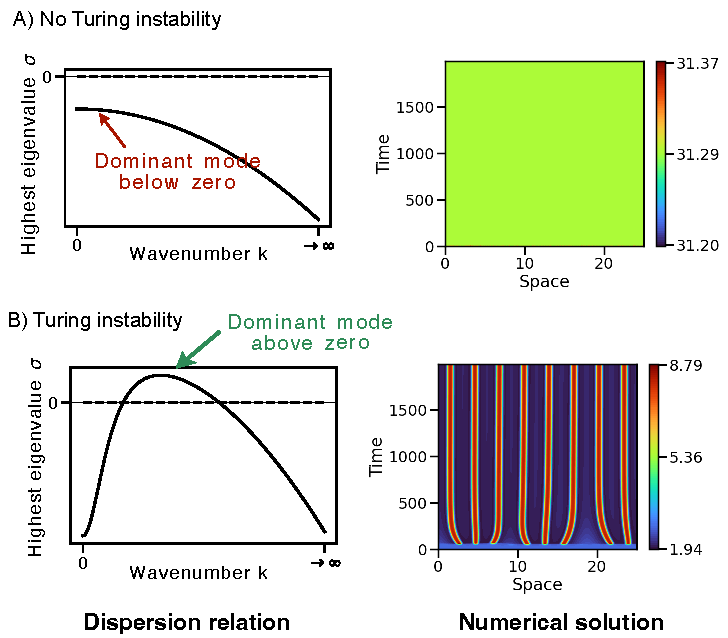
\includegraphics[width=1\textwidth]{chapters/Chapter 1/turing_vs_noturing} % The name of your image file; assumes it's in the same directory as your .tex file
    \caption{A sample caption for the image.}
    \label{fig:turing_vs_noturing} % A label for referencing this figure later in the document
\end{figure}


\subsection{Infering wavelength and convergence time from dispersion relation}


\begin{figure}[H] % h! is a placement specifier; it tries to place the image here.
    \centering
    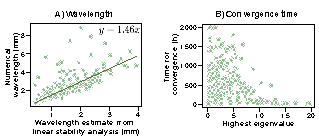
\includegraphics[width=1\textwidth]{chapters/Chapter 1/dispersion_to_wavelength_convergence} % The name of your image file; assumes it's in the same directory as your .tex file
    \caption{A sample caption for the image.}
    \label{fig:dispersion_to_wavelength_convergence} % A label for referencing this figure later in the document
\end{figure}

\subsection{Dispersion to pattern shape}
dispersion to pattern
\begin{figure}[H] % h! is a placement specifier; it tries to place the image here.
    \centering
    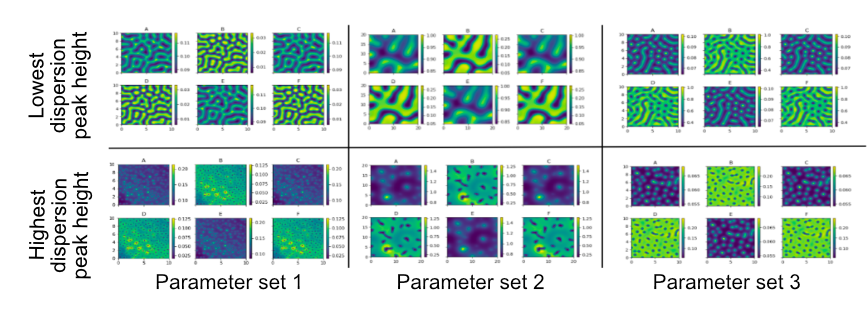
\includegraphics[width=1\textwidth]{chapters/Chapter 1/shape} % The name of your image file; assumes it's in the same directory as your .tex file
    \caption{A sample caption for the image.}
    \label{fig:dispersion_to_shape} % A label for referencing this figure later in the document
\end{figure}



\section{Breaking linear stability analysis predictions}

\subsection{multistability in Turing}
multistaabilityaa
%todo make subfigures bigger
%todo pass all images into pdf


\begin{figure}[H]
%    \begin{adjustbox}{width=1.2\textwidth,center}
        \centering
        \begin{subfigure}{.5\linewidth}
            \centering
            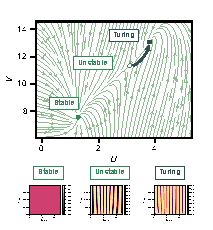
\includegraphics[width=\linewidth]{chapters/Chapter 1/multistability1}
            \caption{First subfigure}
        \end{subfigure}%
        \begin{subfigure}{.5\linewidth}
            \centering
            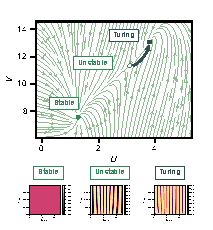
\includegraphics[width=\linewidth]{chapters/Chapter 1/multistability1}
            \caption{Second subfigure}
        \end{subfigure}
        \newline
        \begin{subfigure}{.5\linewidth}
            \centering
            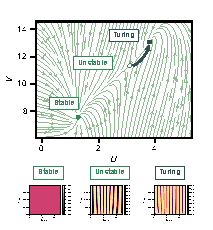
\includegraphics[width=\linewidth]{chapters/Chapter 1/multistability1}
            \caption{Third subfigure}
        \end{subfigure}%
        \begin{subfigure}{.5\linewidth}
            \centering
            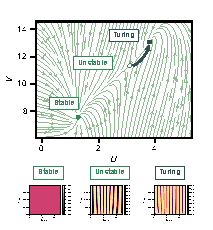
\includegraphics[width=\linewidth]{chapters/Chapter 1/multistability1}
            \caption{Fourth subfigure}
        \end{subfigure}
        \caption{Overall caption for all subfigures}
%    \end{adjustbox}
\end{figure}

%
%\begin{adjustbox}{width=1.4\textwidth,center}
%\begin{figure}
%
%    \caption{(a) blah (b) blah (c) blah (d) blah}
%    \label{fig:foobar}
%
%\end{figure}
%\end{adjustbox}


\subsection{Analytical to numerical: Other types of dispersion relation, and other types of patterns}
 %todo . They also identify examples of non-stationary spatial patterns, when the eigenvalue corresponding to a critical wave number has non-zero imaginary part.Deutsch, A., Dormann, S., et al., 2005. Cellular automaton modeling of biological pattern formation. Springer.

%todo look at pitchfork and transcritical

\begin{figure}[H] % h! is a placement specifier; it tries to place the image here.
    \centering
    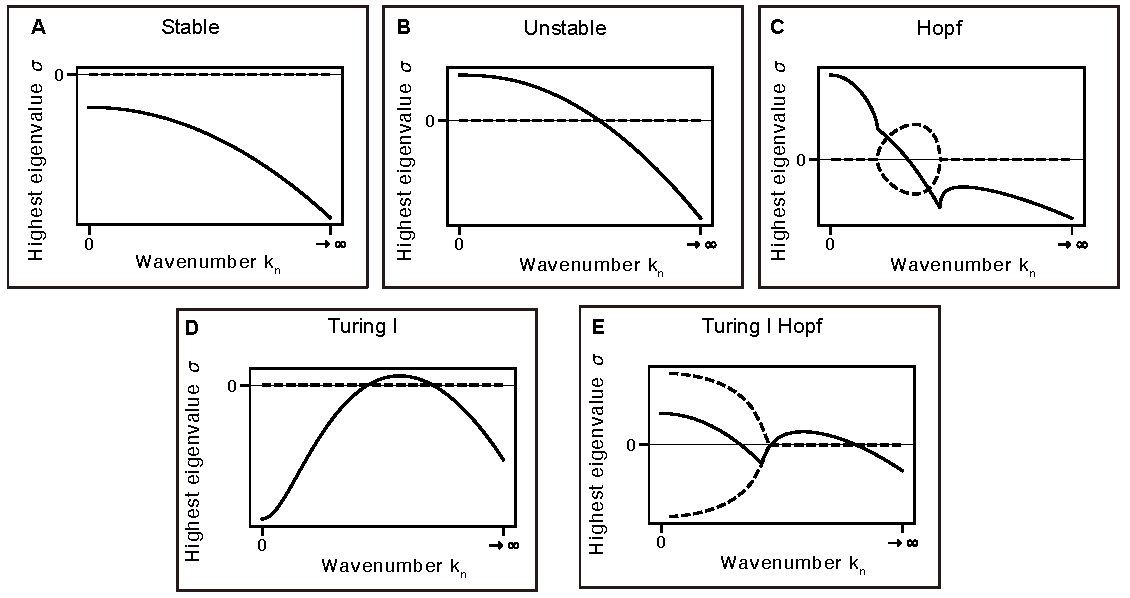
\includegraphics[width=1\textwidth]{chapters/Chapter 1/dispersions} % The name of your image file; assumes it's in the same directory as your .tex file
    \caption{A sample caption for the image.}
    \label{fig:dispersions} % A label for referencing this figure later in the document
\end{figure}

\begin{figure}[H] % h! is a placement specifier; it tries to place the image here.
    \centering
    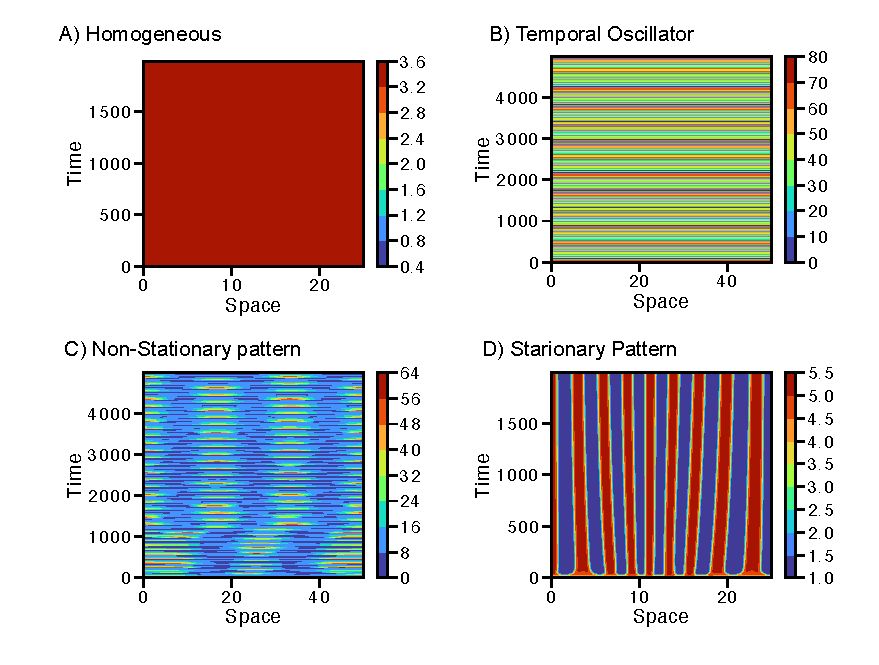
\includegraphics[width=1\textwidth]{chapters/Chapter 1/numerical_patterns} % The name of your image file; assumes it's in the same directory as your .tex file
    \caption{A sample caption for the image.}
    \label{fig:numerical_patterns} % A label for referencing this figure later in the document
\end{figure}

\begin{figure}[H] % h! is a placement specifier; it tries to place the image here.
    \centering
    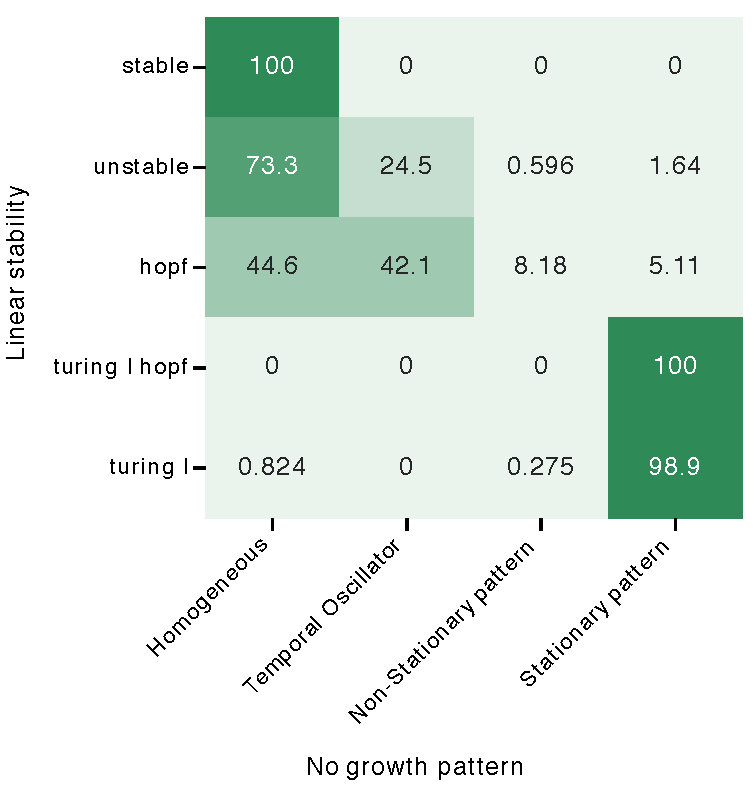
\includegraphics[width=1\textwidth]{chapters/Chapter 1/lsa_numerical_confusion} % The name of your image file; assumes it's in the same directory as your .tex file
    \caption{A sample caption for the image.}
    \label{fig:lsa_numerical_confusion} % A label for referencing this figure later in the document
\end{figure}



\section{Introducing realistic biological phenomena}
\subsection{No growth to open boundaries}
\subsection{Open boundaries to growth}

